\documentclass[tcc]{ic}

\usepackage{indentfirst}
\usetikzlibrary{decorations}
\usetikzlibrary{shapes.symbols}
\usetikzlibrary{shapes.arrows}
\usepackage{icomma}
\usepackage{microtype}
\usepackage[binary-units]{siunitx}
\usepackage{pdfpages}

\newenvironment{demonst} 
               {\noindent \textit{\textbf{Demonstração.}}~ }	% begin demonst
               {\hfill\rule{2mm}{2mm} \vspace{\parskip} } 	% end demonst

\newtheorem{definicao}{Definição}[section]
\newtheorem{teorema}{Teorema}[section]
\newtheorem{lema}{Lema}
\newtheorem{corolario}{Corolário}
\newtheorem{proposicao}{Proposição}

\graphicspath{{../newPlots/}}

%======================================================%
%=========== Informações do documento PDF =============%
%======================================================%
\hypersetup{
colorlinks = {true},
linktocpage = {false},
plainpages = {false},
linkcolor = {Blue},
citecolor = {Blue},
urlcolor = {Red},
unicode = {true},
pdftitle ={Teste para Verificação da Hipótese de Ruído Branco utilizando Teoria da Informação},
pdfauthor = {Marcelo Queiroz de Assis Oliveira},
pdfsubject = {Disserta\c c\~ao de Mestrado},
pdfkeywords={Geradores de Números Aleatórios. Testes Teóricos. Testes Estatísticos. Teoria da Informação.},
pdfcreator = {LaTeX2e},
pdffitwindow = {false},
pdfstartview = {FitH},
pdftoolbar = {true},
pdfpagemode = {UseOutlines},
pdfview = {XYZ null null null}
}

%======================================================%
%================ CAPA DA DISSERTAÇÃO =================%
%======================================================%

\titulo{Teste para Verificação da Hipótese de Ruído Branco utilizando Teoria da Informação}

\autor{Marcelo Queiroz de Assis Oliveira}{marceloqao@gmail.com}{http://sites.google.com/site/marceloqao/}

\orientador{Dr. Alejandro C.\ Frery}{http://sites.google.com/site/acfrery/}{Instituto de Computação}{Universidade Federal de Alagoas}

\orientadorDois{Dr. Heitor Soares Ramos Filho}{https://sites.google.com/a/ic.ufal.br/heitor/}{Instituto de Computação}{Universidade Federal de Alagoas}

\examinador{Dr. Osvaldo Anibal Rosso}{oarosso@gmail.com}{Instituto de Física}{Universidade Federal de Alagoas}

\examinadorDois{Dra.\ Juliana Gambini}{mgambini@itba.edu.ar}{Departamento de Ingeniería Informática}{Instituto Tecnológico de Buenos Aires}

% \examinadorQuatro{Examinador 4}{ex4@email.com}{Instituto ou Departamento}{Universidade do Examinador 4}

\dataMesAno{Novembro}{2017}

\begin{document}

\selectlanguage{portuguese}

\capa

% %======================================================%
% %================= Aprovação - Banca ==================%
% %======================================================%
\newpage
\thispagestyle{empty}
\includepdf[pages=1]{assinaturas_banca.pdf}

% %======================================================%
% %====================== DEDICAÇÃO =====================%
% %======================================================%
 \newpage
 \thispagestyle{empty}
 \mbox{}\vfill
 \begin{flushright}
 À minha amada esposa Élida, aos meus \emph{filhos} Duda, \\
 Gabriel, João Marcelo e Melissa, a minha querida Mãe,\\
 Francisca \textit{(In Memorian)} dedico este trabalho. \\
 Por vocês, faria tudo de novo.
 \end{flushright}

%======================================================%
%======================= RESUMO =======================%
%======================================================%
\begin{resumo}
\noindent 
O nosso ponto de partida é o desejo de analisar
se é viável verificar no plano ($H\times C$), dentro de uma abordagem estatística, se sequências de observações são ruído branco.

Na literatura encontramos diversos trabalhos que fazem isso de forma ``ad hoc'', verificando se o ponto característico de uma sequência nesse plano é próximo ao ponto ($1,0$). 
Contudo, tal como afirma \citet{NewPermutationEntropy}, não encontramos análises detalhadas que permitam atribuir significância estatística a tais afirmações.

Para elucidar essa questão, e diante da impossibilidade de contar com sequências infinitamente longas e que garantidamente sejam ruído branco, coletamos sequências de três fontes diferentes: duas físicas e uma algorítmica considerada de qualidade.
Verificamos se é possível considerá-las ideais para os nossos fins.

Analisamos a dispersão dos pontos característicos dessas sequências no plano ($H\times C$) utilizando quatro fatores: o tamanho da sequência ($N$), o tamanho da palavra ($D$), o \textit{delay} $(\tau)$ e a fonte geradora, observando a distância dos pontos característicos ao ponto de referência. Sugiram então evidências de que a fonte geradora seria um fator irrelevante para a análise.

Com o intuito de consolidar essa possibilidade, aplicamos o teste de Kolmogorov-Smirnov a pares de sequências comparáveis, porém verificamos que apenas duas das fontes geradoras são realmente irrelevantes, as duas fontes físicas.

Agrupamos, então os dados das fontes físicas e passamos a tratá-los como nossa referência, em seguida procuramos por regiões de confiança. 
Adotamos uma abordagem não-paramétrica por não termos nenhuma evidência teórica acerca da distribuição que segue a distância do ponto característico ao de referência quando é analisada uma sequência finita de ruído branco.

Calculamos então os quantis, respeitados os fatores tamanho da sequência ($N$), tamanho da palavra ($D$) e \textit{delay} ($\tau$), que servem como regiões de confiança para o teste que deu origem a este trabalho.

Concluímos a dissertação verificando que sequências produzidas por geradores aceitos pela comunidade geram pontos característicos dentro de regiões de confiança, enquanto que um gerador que foi descartado pelas estruturas que as suas sequências apresentam leva a pontos fora dessas mesmas regiões.
Analisamos também sequências estacionárias e não estacionárias, e para as primeiras fazemos uma análise preliminar do poder do teste.

\vspace{1em}
\noindent {\bf Palavras-chave}: Geradores de Números Aleatórios. Testes Teóricos. Testes Estatísticos. Teoria da Informação.
\end{resumo}

%======================================================%
%====================== ABSTRACT ======================%
%======================================================%
\selectlanguage{english}
\begin{abstract}
\noindent
%Our starting point is the desire to verify in the plane ($H\times C$) in a  statistical approach, if sequences of observations are white noise .

We want to verify  if sequences of observations are white noise  in the plane ($H\times C$).

In the literature, we find several works that do this in an ``ad hoc'' way, checking if the characteristic point of a sequence in that plane is close to the point ($1,0$).

However, as \citet{NewPermutationEntropy} states, we do not found detailed analyzes to assign statistical significance to such statements.

To elucidate this question, and in the face of the impossibility of counting infinitely long sequences that are guaranteed to be white noise, we gather candidate sequences from three different sources: two physical and one algorithmic considered as a good source. We checked, if we may consider them ideals for our purposes.

We analyze the dispersion of the characteristic points of these sequences in the plane ($H\times C$) using four factors: the size of the sequence ($N$), the size of the word ($D$), the delay ($\tau$) and the generating source, observing the distance from the characteristic points to the reference point. We observe that the generating source would be an irrelevant factor to the analyses.

To verify this hipothesis, we applied the Kolmogorov-Smirnov test to pairs of comparable sequences, however we verify that only two sources are equivalents, the both physical.

Therefore, we grouped the data from physical sources, and it became our groundtruth, then in sequence, we searched for trust regions. We adopted a non-parametric approach because we did not have no theoretical evidence about the distribution that follows the distance from the characteristic point to our groundtruth when a finite sequence of white noise candidate is analyzed.

We then calculated the quantiles, respecting the factors sequence size ($N$), size of the word ($D$) and delay ($\tau$), which serve as confidence regions for the test that gave rise to this work.

We conclude the dissertation by verifying that sequences produced by community accepted generators generate characteristic points within confidence regions, while a generator that has been discarded by the structures that its sequences present leads to points outside these regions.
We also applied the test to stationary and nonstationary sequences and, for the former, we make a preliminary assessment of the test power.

\vspace{1em}
\noindent 
{\bf Keywords}: Random Number Generators. Theoretical tests. Statistical Tests. Information theory.
\end{abstract}

%======================================================%
%=================== AGRADECIMENTOS ===================%
%======================================================%
\selectlanguage{portuguese}
\begin{agradecimentos}
\noindent

A Deus pelo dom da vida e por manter-me são durante o desenvolvimento deste trabalho.

A meus Pais pelos ensinamentos que não temos dentro da escola e pelo incentivo a buscar o aperfeiçoamento intelectual.

A minha esposa Elida, pelo companheirismo em tudo!

A meus filhos, Maria Eduarda, Gabriel, João Marcelo e Melissa, por sua enorme alegria de viver e seu sorriso.

Aos colegas do mestrado, com os quais vivi frutíferos e divertidos momentos de estudo, valeu Rodrigo, Domarques, Davy, 
Felipe, Brião, Pedro, Torres e todos os colegas do curso e do LaCCAN.

Ao colega Joao Borges pela grande contribuição na implementação.

Ao Professor Christoph Marquardt do \textit{Max Planck Institute for the Science of Light} e ao Professor Mads Haahr do \textit{Trinity College Dublin} e criador do \textit{www.random.org} pela gentileza em fornecer dados realmente aleatórios, sem os quais este trabalho não teria sido realizado.

A todos os colegas da UFAL que direta ou indiretamente contribuiram para este trabalho, no LCCV, NTI e na gesão central da universidade, em especial ao companheiro Kleymerson por segurar a barra durante os momentos finais e também à Magnífica Reitora da UFAL, Valéria Correia e José Vieira, Vice Reitor. E ainda a todos que sempre inquiriam acerca do desenvolvimento deste trabalho.

Aos servidores do Instito de Computação da UFAL, em especial Vitor Torres pela presteza e atenção em atender os alunos do curso de Mestrado em Modelagem Computacional de Conhecimento, da mesma forma aos professores do curso.

Ao professor Osvaldo Rosso pela imensa contribuição relativa à teoria da informação e pelas ricas conversas acerca do tema

E finalmente aos meus orientadores, Alejandro Frery e Heitor Ramos sem os quais este trabalho não teria se concretizado, obrigado pelo incentivo, pela disponibilidade e pela paciência. 

Muito obrigado!!

\vspace{1em}
\begin{flushright}
Marcelo Queiroz de A. Oliveira
\end{flushright}
\end{agradecimentos}

%======================================================%
%====================== EPÍGRAFE ======================%
%======================================================%
% \newpage
% \thispagestyle{empty}
% \mbox{}\vfill
% \begin{flushright}
% \emph{``frase.''}\\
% \vspace{1em}
% \textbf{Autor}
% \end{flushright}

%======================================================%
%======================= LISTAS =======================%
%======================================================%
\mylistoffigure

\mylistoftable

% \mylistofalgorithm

%\mylistofequation

\mylistofcontents

\inicio
\setcounter{page}{9} %verificar quantas páginas possuem até iniciar o capítulo 1 (subtraindo capa, folha de aprovação e catalogação).


%\mychapter{Introdução}{chp:introducao}
\lhead{INTRODUÇÃO}

  \lettrine{}{} 

\section{Motivação}
  
%   \lettrine{N}{a} .


\section{Visão geral}



%\section{Contribuições}

%   O trabalho proposto visa contribuir no tocante à sobrevida de Redes de Sensores sem Fios, aumentando o tempo de funcionamento das mesmas através da maior disponibilidade de energia nos nós que a constituem. O trabalho se apoia na estabilidade, desempenho e confiabilidade da linguagem R \citep{R} fazendo uso das boas práticas de \emph{Reproducible Research} como apresentadas em \citet{RR2010}.


%\section{Riscos}

%   Há riscos envolvidos no processo Científico aqui tratado, dentre eles, pode-se citar

\begin{center}
	\fbox{
	\colorbox[RGB]{227, 227, 227}{
	\parbox[t]{.8\linewidth}
		{Neste capítulo foram tratados os aspectos introdutórios ao tema como a motivação e uma visão geral do mesmo, no próximo capítulo é feita uma fundamentaćão teórica visando fundamentar a idéias propostas no trabalho.}} }
\end{center}

% % % Aprender Git!
\mychapter{Introdução e Delimitação do Problema}{chp:Fundamentação Teórica}
\lhead{Introdução e Delimitação}

% Breve resumo do capítulo.
\lettrine{E}{ste} capítulo tem como objetivo apresentar uma fundamentação teórica necessária para embasar os conceitos aplicados no trabalho.
Delimitaremos aqui o problema a ser tratado nesta tese.

Em relação a fundamentação teórica, utilizou-se como principal fonte de pesquisa a área de indexação de periódicos científicos ISI \emph{Web of Knowledge}, onde foram obtidas a grande maioria das referências, usando como parâmetros o fator de impacto dos periódicos pesquisados, a quantidade de citações de cada publicação, o grau de relevância para o tema pesquisado e o nível de produtividade (fator-H) dos autores envolvidos. 
O apoio em livros, \textit{surveys}, \textit{lecture notes} e ferramentas complementares de busca, como o \emph{Google Acadêmico} foram utilizadas para complementar esta pesquisa.

\section{Números Aleatórios} %Simulação física, Von Neumann, Congruenciais Lineares, etc

A noção de aleatoriedade é fundamental em diversas áreas, entretanto uma definição precisa, até mesmo do ponto de vista matemático rigoroso, é bastante difícil. 
Algumas questões emergem naturalmente como, o que vem a ser aleatoriedade? 
Existem eventos aleatórios na natureza? 
Faz algum sentido buscar leis da aleatoriedade? 
É possível simular a aleatoriedade? 
Estas são questões muito difíceis, envolvendo, inclusive, os primórdios da investigação filosófica como discute \citep{Volchan:02}.
Essa dificuldade é bem ilustrada de forma humorística na Figura~\ref{fig:Dilbert}.

\begin{figure}[hbt]
\centering
\includegraphics[width=.7\linewidth]{dilbert}
\caption{Visão de Dilbert de um gerador de números aleatórios}\label{fig:Dilbert}
\end{figure}

Números aleatórios perfazem uma das partes mais importantes em aplicações computacionais nos vários campos do conhecimento, como aborda \citep{Knuth:98}:
\begin{itemize}
     \item \textit{Simulação} - Quando um computador é usado para simular fenômenos naturais, números aleatórios são necessários para fazer as coisas de forma realística. Simulação abrange diversas áreas, desde o estudo de física nuclear (onde particulas são submetidas a colisões aleatórias) até pesquisa operacional (como, por exemplo, a taxa de pessoas que entram num aeroporto em intervalos aleatórios).
     \item \textit{Amostragem} - É praticamente impossível examinar todos os possíveis casos, porém uma amostra aleatória provê um palpite sobre como é o comportamento típico do fenômeno em questão.
     \item \textit{Análise Numérica} - Técnicas elaboradas para a solução de complexos problemas numéricos foram desenvolvidas utilizando-se números aleatórios.
     \item \textit{Programação de Computadores} - Valores aleatórios são uma ótima fonte de dados para testar a eficácia de algoritimos computacionais.
     \item \textit{Tomada de Decisão} - Existem relatos de que diversos executivos tomam suas decisões lançando moedas ou atirando dardos. Também há rumores de que professores universitários lançam suas notas de forma similar. Em alguns momentos é importante tomar decisões de forma não influenciada por qualquer agente externo.
     \item \textit{Criptografia} - Uma fonte de bits não viesada é essencial para diversos tipos de comunicações seguras, quando os dados precisam ser mantidos em sigilo.
     \item \textit{Estética} - Um pouco de aleatoriedade faz com que gráficos e músicas geradas por computador aparentem ser menos artificiais.
     \item \textit{Diversão} - Rolar dados, embaralhar cartas, girar rodas de roletas, etc., são passatempos facinantes para muitos. Estes usos tradicionais de números aleatórios sugeriram o nome ``Método de Monte Carlo''.
    \end{itemize}

Existem dois tipos básicos de geradores utilizados para produzir sequências aleatórias: GNAs -- Geradores de Números Aleatórios, do inglês (\textit{RNGs} -- \textit{Random Number Generators}) e GNPA -- Geradores de Números Pseudoaleatórios, do inglês (\textit{PRNGs} -- Pseudorandom Number Generators).

\subsection{Geradores de Números Aleatórios -- GNA}
  
Geradores de Números Aleatórios utilizam uma fonte não determinística juntamente com algumas funções de processamento para produzir aleatoriedade. 
As saídas deste tipo de gerador podem ser usadas diretamente como números aleatórios, desde que satisfaçam critérios de aleatoriedade, ou ainda podem servir como parâmetro de entrada para geradores de números pseudoaleatórios, vistos com mais detalhes na sequência. 

A maior parte dos geradores utiliza-se de fenômenos físicos naturais como, decaimento radioativo, ruidos termais em semiconcutores, amostras de som num local ruidoso, ruído no espectro eletromagnético, dentre outros que, por óbvia dedução, carecem de algum hardware específico para serem capturados. 

Na literatura é possível encontrar trabalhos relatando detalhadamente a criação de geradores de números aleatórios utilizando fontes de aleatoriedade apropriadas.
\citet{Fairfield:85} descrevem a geração de um fluxo de bits aleatórios baseado na instabilidade da frequência de um oscilador.
Evidentemente a construção de um gerador como o descrito anteriormente demanda o emprego de técnicas apuradas e um grande conhecimento teórico, além de necessitar, em sua grande maioria, de hardware especializado, o que gera uma barreira para os usuários que demandam tais dados aleatórios.
Desta sorte, frequentemente os usuários precisam se valer de técnicas alternativas para obter aleatoriedade.

\subsection{Geradores de Números Pseudoaleatórios -- GNPA}

Dadas as dificuldades descritas anteriormente, atualmente a maneira mais conveniente e confiável de se gerar números aleatórios para diversas aplicações é através de algoritmos com um sólido embasamento matemático. 
Tais algoritmos produzem sequências de números sabidamente não aleatórios ao todo, mas que aparentam comportar-se como números aleatórios independentes, isto é, tomada uma sequência de variáveis aleatórias independentes e identicamente distribuídas sobre o Intervalo $(0,1)$. 
Tal sequência pode ser chamada de ``Pseudoaleatória'' e o programa utilizado em sua produção de ``Gerador de Números Pseudoaleatórios'' como define \citet{LEcuyer:98}.

\section{Principais Testes Clássicos} %Revisão Cronológica/Conceitual

Existem duas abordagens para testar-se a capacidade de geradores aleatórios ou pseudoaleatórios produzirem sequências ditas aleatórias.
Segundo \citet{LEcuyer:92} são elencados em teóricos e empíricos.

Os testes teóricos são bastante específicos para cada tipo de GNPA, pois analisam o as propriedades das sequências a partir da definição do gerador.
Já os testes empíricos valem-se de técnicas estatísticas objetivando avaliar o quão boas são as sequências produzidas por um determinado gerador.
Estes últimos podem ser aplicados tanto a GNAs quanto a GNPAs.

Neste trabalho propomos um teste empírico não paramétrico baseado em ferramentas da teoria da informação.
A seguir daremos uma breve introdução aos testes disponíveis na literatura e ao estado da arte.
  
% \subsection{Diehard}
 
 \subsection{NIST}
 
Fundado em 1991, o NIST (\textit{National Institute of Standards and Technology}) é uma agência não regulatória do Departamento de Comércio dos Estados Unidos da América que tem por missão promover a inovação e a competitividade nos EUA através da ciência de medidas, padrões e tecnologia de forma a alavancar a segurança econômica e melhorar a qualidade de vida do povo americano.

A sua Divisão de Segurança de Computadores (CSD) e o Centro de Pesquisa em Segurança Computacional (CSRC) facilitam a ampla disseminação de práticas e ferramentas de segurança da informação, provendo recursos para a definição de padrões além de identificar recursos de segurança na Web para suportar usuários na industria, governo e academia. 

CSRC é o portal de acesso primário para se ter acesso às publicações de segurança de computadores, padrões e instruções, além de outras informações relacionadas a segurança.

Desde 1997, o Grupo de Trabalho Técnico em Geração de Números Aleatórios (RNG-TWG) tem trabalhado no desenvolvimento de uma bateria de testes estatísticos apropriados para a avaliação de geradores de números aleatórios e pseudoaleatórios utilizados em aplicações criptográficas. 

Os principais objetivos do grupo são:
  \begin{itemize}
   \item Desenvolvimento de uma bateria de testes estatísticos para detectar não aleatoriedade em sequencias binárias construidas através de geradores de números aleatórios e pseudoaleatórios utilizados em aplicações criptográficas;
   \item Produzir documentação e uma implementação em software destes testes;
   \item Prover auxílio no uso e aplicação destes testes.
  \end{itemize}

\subsection{Diehard e Dieharder}

George Marsaglia desenvolveu a bateria de testes Diehard em 1995, e os disponibilizou em CD-ROM.
Robert Brown identificou limitações nessa bateria de testes, os implementou novamente na linguagem de programação C, acrescentou testes da bateria NIST e disponibilizou um conjunto ampliado de testes denominado Dieharder.
A página Web \url{http://webhome.phy.duke.edu/~rgb/General/dieharder.php} é o portal de acesso a esses testes bem como a resultados de aplicá-los a diversas fontes de dados.

\subsection{ENT}

ENT \citet{ENTTestSuite} realiza uma variedade de testes no fluxo de bytes de um arquivo (ou na entrada padrão se nenhum arquivo for especificado) e produz uma saída como esta:

\begin{verbatim}
Entropy = 7.980627 bits per character.

Optimum compression would reduce the size
of this 51768 character file by 0 percent.

Chi square distribution for 51768 samples is 1542.26, and randomly
would exceed this value less than 0.01 percent of the times.

Arithmetic mean value of data bytes is 125.93 (127.5 = random).
Monte Carlo value for Pi is 3.169834647 (error 0.90 percent).
Serial correlation coefficient is 0.004249 (totally uncorrelated = 0.0).
\end{verbatim}

ENT é distribuido em forma de binário para a plataforma Win32 e pode ter descarregado o seu código fonte para construção sob ambiente \textit{Unix-Like}
  
\subsection{TestU01}	

Considerado como o estado da arte dos testes para geradores de números aleatórios \citet{LEcuyer:07}, o $TestU01$ se apresenta como uma biblioteca de software escrita em $ANSI$ $C$ que oferece uma coleção de utilitários para testagem, ele provê implemetações generalistas dos testes estatísticos clássicos para geradores de números aleatórios, bem como de vários outros propostos na literatura, além de propor alguns originais. Pode ser aplicado a números aleatórios produzidos por qualquer tipo de dispositivo ou armazenados em arquivos.

O principal problema com o uso dos testes NIST, Dieharder, Test$U01$ e outros similares é que estão direcionados a usuários especializados.
Uma parcela significativa de pesquisadores prefere ferramentas visuais, como a descrita a seguir.

\subsection{Visualização}

O intuito desses testes é a verificação de que os dados produzidos por um gerador, seja ele algoritmico ou físico, não se afastam significativamente da hipótese de serem eventos de variáveis independentes e identicamente distribuídas segundo uma lei Uniforme no intervalo $(0,1]$.

Verificar que os dados seguem uma lei Uniforme é relativamente simples, e há para eles uma bateria de testes que observam diversas propriedades.

A componente mais difícil é a de verificar a independência, por se tratar de independência coletiva e não apenas aos pares.

A falta de independência de uma sequência de $N$ pontos pode se manifestar de várias maneiras.
Uma delas é quando os pontos jazem em subespaços de dimensão menor a $N$, ao invés de preencher o espaço por completo.

As figuras~\ref{fig:3DMT} e~\ref{fig:3DRandu} mostram sequências de três pontos não sobrepostos desenhadas no cubo unitário.
A primeira perspectiva (figs.~\ref{MTa} e~\ref{Ra}) mostram uma perspectiva dos pontos que não levanta nenhuma suspeita.
Já as figuras~\ref{MTb} e~\ref{Rb} mostram que as sequências produzidas pelo gerador RANDU não preenchem o espaço, mas ficam confinadas a alguns planos, enquanto que as produzidas por Mersenne-Twister não apresentam essa deficiência.

\begin{figure}[hbt]
\centering
\subfigure[Primeira perspectiva\label{MTa}]{\includegraphics[width=.48\linewidth]{MT3D}}
\subfigure[Segunda perspectiva\label{MTb}]{\includegraphics[width=.48\linewidth]{MT3Dsubspace}}
\caption{Visualização 3D de sequências disjuntas produzidas pelo gerador Mersenne-Twister}\label{fig:3DMT}
\end{figure}

\begin{figure}[hbt]
\centering
\subfigure[Primeira perspectiva\label{Ra}]{\includegraphics[width=.48\linewidth]{Randu3D}}
\subfigure[Segunda perspectiva\label{Rb}]{\includegraphics[width=.48\linewidth]{Randu3Dsubspace}}
\caption{Visualização 3D de sequências disjuntas produzidas pelo gerador RANDU}\label{fig:3DRandu}
\end{figure}

Embora o exemplo mostre claramente que o gerador RANDU apresenta problemas, nem sempre é fácil identificar esse tipo de estrutura.
Isso se deve a que ela pode ocorrer em espaços de dimensão maior, ou seguindo estruturas mais complexas.

\subsection{Descritores baseados em Teoria da Informação}

O trabalho pioneiro de \citet{PermutationEntropyBandtPompe} representa uma mudança de paradigma na análise de séries temporais, e será o nosso marco referencial teórico.

Eles propõem uma técnica não-paramétrica de análise de sequências que consiste em transformar palavras de $D$ dados não necessariamente subsequentes em símbolos ordinais.
Esses símbolos codificam a ordem que as $D$ observações têm na sequência e, portanto, são bem menos sucetíveis a contaminação dos que os próprios valores.
Forma-se então um histograma de proporções dos símbolos observados, e calculam-se duas quantidades: a Entropia e a Divergência de Jensen-Shannon a uma distribuição de referência (usualmente a uniforme).
A série, finalmente, é representada pelo par de valores Entropia-Complexidade Estatística, sendo que esta última é o produto da Entropia e a Divergência de Jensen-Shannon.

O conjunto de valores possíveis dos pontos característicos de qualquer série não varre $\mathbbm R^2$, mas constitui-se em um subconjunto compacto do plano: o plano Entropia-Complexidade, visto na Figura \ref{fig:Plano_HC}.
\begin{figure}[hbt]
	\centering
	\includegraphics[width=.7\linewidth]{plano_HC}
	\caption{Plano Entropia-Complexidade.}\label{fig:Plano_HC}
\end{figure}
Uma grande quantidade de trabalhos mostra que a posição dos pontos característicos no plano Entropia-Complexidade é capaz de caracterizar diversos tipos de dinâmicas, sendo as duas extremas o ponto $(0,0)$, que corresponde a sequências determinísticas, e o ponto $(1,0)$, típico de ruído branco.

Alguns dos trabalhos emblemáticos que empregam essa abordagem são:
\begin{description}
\item[\citet{RandomNumberGeneratorsCausality}] mostram que o plano Entropia-Complexidade permite prever o resultado dos testes Diehard de qualidade de GNPA.
\item[\citet{GeneralizedStatisticalComplexityMeasuresGeometricalAnalyticalProperties}] analisam o mapa caótico logístico e discutem cotas no plano Entropia-Complexidade.
\item[\citet{EEGAnalysisWaveletInformationTools}] analisam dados de eletroencefalogramas de pacientes com epilepsia 	utilizando decomposição wavelet e o plano Entropia-Complexidade.
\item[\citet{De_Micco_2008}] avaliam melhorias da qualidade de sequências pseudoaleatórias.
\item[\citet{De_Micco_2009}] estudam as componentes caóticas de GNPAs.
\item[\citet{ComplexNetworksEvolution}] analisam a evolução de redes dinâmicas com descritores baseados em Teoria da Informação.
\item[\citet{DistinguishingChaoticStochasticDynamicsTimeSeriesMultiscaleSymbolicApproach}] analisam a relação entre dinâmicas caóticas e estocásticas com uma abordagem multiescala.
\item[\citet{StructuralChangesDataCommunicationWSN}] utilizam descritores de Teoria da Informação para descrever a dinâmica de redes de sensores sem fios.
\item[\citet{DistinguishingNoiseFromChaos}] caracterizam sequências com componentes caóticas e estocásticas no plano Entropia-Complexidade.
\item[\citet{CharacterizationVehicleBehaviorInformationTheory}] analisam o comportamento de veículos em larga escala em função da topologia de diversas cidades.
\item[\citet{DiagnosingDynamicsObservedSimulatedEcosystem}] analisam séries temporais de fenômenos ambientais.
\item[\citet{InformationTheoryPerspectiveNetworkRobustness}] verificam o efeito de ataques em redes complexas através de descritores no plano Entropia-Complexidade.
\item[\citet{ClassificationVerificationOnlineHandwrittenSignatures}] mostram a expressividade dos descritores de Teoria da Informação para o problema de classificação e verificação de assinaturas.
\item[\citet{CharacterizationElectricLoadInformationTheoryQuantifiers}] conseguem caracterizar o tipo de dispositivo elétrico observando o ponto no plano Entropia-Complexidade em que o histórico do seu consumo é mapeado.
\end{description}

Uma limitação de todos esses trabalhos é que os pontos no plano são atribuídos a padrões prototípicos, isto é, a modelos, de forma \textit{ad hoc}.
O autor desta dissertação só conhece um trabalho em que é feita uma análise da significância da posição de pontos característicos no plano Entropia-Complexidade: o artigo de \citet{NewPermutationEntropy}.

Nesse contexto, esta dissertação fornece regiões de confiança para uma boa diversidade de situações que permitem verificar a significância da hipótese de uma sequência aleatória ou pseudoaleatória é aderente à hipótese dela ser ruído branco.

\section{Delimitação do problema} %Delimitação do problema  

A motivação deste trabalho é o desenvolvimento de um teste baseado em Teoria da Informação para verificar a hipótese de que uma sequência é ruído branco, isto é, formada por observações de variáveis aleatórias independentes e identicamente distribuídas.
Para tanto, trabalharemos com atributos derivados da simbolização de Bandt \& Pompe.
Cada sequência sob análise será transformada em um ponto no plano Entropia-Complexidade, e será medida a sua distância ao ponto característico de sequências ideais.
Analisaremos, então, a distribuição empírica de uma variedade de situações de interesse para, finalmente, propor regiões de confiança da hipótese nula.
Por fim, analisaremos sequências com o ferramental aqui proposto.

\include{./capitulos/03-proposta}
\mychapter{Resultados}{chp:resultados}
\lhead{RESULTADOS}


Trabalhamos com sequências de observações provindas de três geradores: dois físicos (considerados ``verdadeiramente aleatórios'') e um algorítmico (o gerador Mersenne-Twister, que é reputado um dos melhores geradores pseudoaleatórios).

Para cada gerador considerado coletamos sequências disjuntas de tamanho \num{1000} e \num{50000}, de cada tamanho de palavra $D$ e a cada \textit{lag} $\tau$.
Temos, assim, quatro fatores a serem analisados.

Cada sequência passou pelo processo de simbolização, e foi calculado o histograma dos símbolos.
Foram então calculados os valores de Entropia e de Complexidade de cada histograma, bem como a distância euclidiana desses valores ao ponto de referência $(1,0)$.

O primeiro passo consistiu em fazer uma análise visual das distâncias dentro do plano $(H,C)$.
Dessa análise visual concluímos que é plausível eliminar o fator gerador e, para tanto, aplicamos o teste de Kolmogorov-Smirnov aos pares de distâncias oriundas de distâncias comparáveis, isto é, provindas dos mesmo fatores $N$, $D$ e $\tau$.

Os testes de Kolmogorov-Smirnov não nos fazem rejeitar a hipótese de que os diferentes geradores produzem sequências com idênticas propriedades no que diz respeito à distância ao ponto de referência.
Assim, nos passos seguintes analisamos o agregado das distâncias provindas dos três geradores considerados.

Acompanhando a análise realizada por \citet{NewPermutationEntropy}, calculamos os quantis de ordem $999/1000$, $1/100$, $5/100$ e $10/100$ das distâncias agrupadas pelos fatores relevantes ($N$, $D$ e $\tau$).
Com isso, produzimos intervalos de confiança para testar a hipótese de que a
distância do ponto característico de uma sequência é compatível com a de uma sequência de ruído branco.
No repositório associado a esta dissertação deixamos disponíveis as funções de distribuição acumuladas dessas distâncias, com as quais é possível calcular o $p$-valor, e não apenas a decisão binária ``rejeita'' ou ``não rejeita''.

\section{Análise global das sequências}

Em todos os casos os pontos foram desenhados com \SI{1}{\percent} de transparência, para evidenciar as regiões mais e menos densas.

As figuras~\ref{Fig:ScatterAll_Quant_1k} e~\ref{Fig:ScatterAll_Quant_50k} mostram os planos Entropia-Complexidade com as respectivas curvas de complexidade mínima e máxima para cada par $D\in\{3, 4, 5, 6\}$ (colunas) e $\tau\in\{1, 10, 30, 50\}$ (linhas), com os \num{52429} pontos observados a partir das sequências obtidas pelo gerador quântico tomando $1.000$ e $50.000$ sequências respectivamente.


\begin{figure}[hbt]
	\centering
	\includegraphics[width=\linewidth]{ScatterAll_Quant_1k}
	\caption{Diagramas de dispersão das sequências quânticas com $1.000$ observações para $D\in\{3, 4, 5, 6\}$ (colunas) e $\tau\in\{1, 10, 30, 50\}$ (linhas), com curvas de complexidade mínima e máxima no plano Entropia-Complexidade.}\label{Fig:ScatterAll_Quant_1k}
\end{figure}

\begin{figure}[hbt]
	\centering
	\includegraphics[width=\linewidth]{ScatterAll_Quant_50k}
	\caption{Diagramas de dispersão das sequências quânticas com $50.000$ observações para $D\in\{3, 4, 5, 6\}$ (colunas) e $\tau\in\{1, 10, 30, 50\}$ (linhas), com curvas de complexidade mínima e máxima no plano Entropia-Complexidade.}\label{Fig:ScatterAll_Quant_50k}
\end{figure}

As figuras~\ref{Fig:ScatterAll_Radio_1k} e~\ref{Fig:ScatterAll_Radio_50k} mostram os planos Entropia-Complexidade com as respectivas curvas de complexidade mínima e máxima para cada par $D\in\{3, 4, 5, 6\}$ (colunas) e $\tau\in\{1, 10, 30, 50\}$ (linhas), com os \num{52429} pontos observados a partir das sequências obtidas pelo gerador de rádio tomando $1.000$ e $50.000$ sequências respectivamente.


\begin{figure}[hbt]
	\centering
	\includegraphics[width=\linewidth]{ScatterAll_Radio_1k}
	\caption{Diagramas de dispersão das sequências de rádio com $1.000$ observações para $D\in\{3, 4, 5, 6\}$ (colunas) e $\tau\in\{1, 10, 30, 50\}$ (linhas), com curvas de complexidade mínima e máxima no plano Entropia-Complexidade.}\label{Fig:ScatterAll_Radio_1k}
\end{figure}

\begin{figure}[hbt]
	\centering
	\includegraphics[width=\linewidth]{ScatterAll_Radio_50k}
	\caption{Diagramas de dispersão das sequências de rádio com $50.000$ observações para $D\in\{3, 4, 5, 6\}$ (colunas) e $\tau\in\{1, 10, 30, 50\}$ (linhas), com curvas de complexidade mínima e máxima no plano Entropia-Complexidade.}\label{Fig:ScatterAll_Radio_50k}
\end{figure}

As figuras~\ref{Fig:ScatterAll_MT_1k} e~\ref{Fig:ScatterAll_MT_50k} mostram os planos Entropia-Complexidade com as respectivas curvas de complexidade mínima e máxima para cada par $D\in\{3, 4, 5, 6\}$ (colunas) e $\tau\in\{1, 10, 30, 50\}$ (linhas), com os \num{52429} pontos observados a partir das sequências obtidas pelo gerador Mersenne-Twister tomando $1.000$ e $50.000$ sequências respectivamente.

\begin{figure}[hbt]
	\centering
	\includegraphics[width=\linewidth]{ScatterAll_MT_1k}
	\caption{Diagramas de dispersão das sequências de Mersenne-Twister com $1.000$ observações para $D\in\{3, 4, 5, 6\}$ (colunas) e $\tau\in\{1, 10, 30, 50\}$ (linhas), com curvas de complexidade mínima e máxima no plano Entropia-Complexidade.}\label{Fig:ScatterAll_MT_1k}
\end{figure}

\begin{figure}[hbt]
	\centering
	\includegraphics[width=\linewidth]{ScatterAll_MT_50k}
	\caption{Diagramas de dispersão das sequências de Mersenne-Twister com $50.000$ observações para $D\in\{3,4,5,6\}$ (colunas) e $\tau\in\{1,10,30,50\}$ (linhas), com curvas de complexidade mínima e máxima no plano Entropia-Complexidade.}\label{Fig:ScatterAll_MT_50k}
\end{figure}

A olho nu, $D$ é um fator relevante pois os diagramas de dispersão mostram comportamentos que merecem uma análise mais aprofundada, por outro lado não temos certeza de como $\tau$ e o gerador influenciam os resultados. 

As figuras~\ref{fig:GeradorIrrelevante1k} e~\ref{fig:GeradorIrrelevante50k} mostram os histogramas suavizados das distâncias para sequências de tamanho ($N=1.000$, $50.000$) respectivamente, com palavras de tamanho $D=6$  e valores de \textit{lag} ($\tau=1, 50$), sobrepondo os três geradores.
Os gráficos sugerem que o gerador é um fator irrelevante para a distribuição da distância.
Mais adiante veremos que esta impressão não se confirma totalmente.

\begin{figure} %D=6 %N 1000 t1 t 50
	\centering
		\subfigure[$D=6, \tau=1$]{\includegraphics[width=.48\linewidth]{Hist_D6_1k_t1}}
		\subfigure[$D=6, \tau=50$]{\includegraphics[width=.48\linewidth]{Hist_D6_1k_t50}}
		\caption{Histogramas suavizados de situações que sugerem que o gerador é um fator irrelevante para $N=1.000$}\label{fig:GeradorIrrelevante1k}
\end{figure}

\begin{figure} %D=6 %N 50000 t1 t 50
	\centering
		\subfigure[$D=6, \tau=1$]{\includegraphics[width=.48\linewidth]{Hist_D6_50k_t1}}
		\subfigure[$D=6, \tau=50$]{\includegraphics[width=.48\linewidth]{Hist_D6_50k_t50}}
		\caption{Histogramas suavizados de situações que sugerem que o gerador é um fator irrelevante também para $N=50.000$}\label{fig:GeradorIrrelevante50k}
\end{figure}

A figura~\ref{fig:NRelevante} mostra os histogramas suavizados das distâncias dos três geradores para palavras de tamanho $D=6$ e dois valores de \textit{lag} ($\tau=1$, $50$), sobrepondo os resultados obtidos com os dois tamanhos de sequências ($N=1.000$, $50.000$).
Os gráficos sugerem fortemente que o tamanho das sequências é um fator relevante para a distribuição da distância.

\begin{figure} %D=6 %t 1 N 1000 N 50000 (três geradores) %t 50 N 1000 N 50000 (três geradores)
	\centering
		\subfigure[$D=6$, $\tau=1$]{\includegraphics[width=.48\linewidth]{Hist_D6_t1}}
		\subfigure[$D=6$, $\tau=50$]{\includegraphics[width=.48\linewidth]{Hist_D6_t50}}
	\caption{Histogramas suavizados de situações que sugerem que o $N$ é um fator relevante}\label{fig:NRelevante}
\end{figure}

A figura~\ref{fig:DRelevante} mostra os histogramas suavizados das distâncias dos três geradores para dois tamanhos de sequências ($N=1.000$, $50.000$) e dois valores de \textit{lag} ($\tau=1$, $50$), sobrepondo os resultados obtidos com os diferentes tamanhos de palavras ($D=3$, $4$, $5$, $6$).
Os gráficos sugerem fortemente que o tamanho das palavras é um fator relevante para a distribuição da distância.

\begin{figure} %t 1 N 1000, D 3 D 4 D 5 D 6 %t 50 N 50000, D 3 D 4 D 5 D 6
	\centering
		\subfigure[$\tau=1$, $D=1.000$]{\includegraphics[width=.48\linewidth]{Hist_t1_1k}}
		\subfigure[$D=6$, $\tau=50$]{\includegraphics[width=.48\linewidth]{Hist_t50_50k}}
	\caption{Histogramas suavizados de situações que sugerem que o $D$ é um fator relevante}\label{fig:DRelevante}
\end{figure}



\begin{figure} %D 6 %N 1000, t 1 t 10 t 30 t 50 %N 50000, t 1 t 10 t 30 t 50
	\centering
	\subfigure[$\tau=1$, $D=1.000$]{\includegraphics[width=.48\linewidth]{Hist_D6_1k}}
	\subfigure[$D=6$, $\tau=50$]{\includegraphics[width=.48\linewidth]{Hist_D6_50k}}
\caption{Histogramas suavizados de situações que sugerem que o $\tau$ é um fator relevante}\label{fig:tRelevante}
\end{figure}

Para consolidar esta análise realizamos a seguir testes Kolmogorov-Smirnov afim de analisar a influência dos fatores envolvidos nesta análise.

A Tabela~\ref{tab:KS_1000} mostra os $p$-valores dos testes de Kolmogorov-Smirnov aplicados a pares de distâncias calculadas sobre sequências de tamanho $1000$, variando $D$ e $\tau$.
Verificamos que há excelente aderência entre os pares de distâncias de sequências Quânticas e de Rádio.
Já quando a comparação é feita com distâncias de sequências de Mersenne-Twister (M-T), a aderência diminui um pouco.

\begin{table}[hbt]
	\centering
	\caption{Teste de Kolmogorov-Smirnov aplicado a pares de sequências para $1.000$ observações.}\label{tab:KS_1000}
	\begin{tabular}{cccccc}
		\toprule
		Par  &    $D$ & $\tau=1$   &   $\tau=10$   &   $\tau=30$   &   $\tau=50$   \\ \midrule
Quântica vs.\ Rádio		& $D=3$ & 0.18034676 & 0.08582490 & 0.58096350 & 0.32626542 \\
		& $D=4$ & 0.21708776 & 0.60690204 & 0.08116764 & 0.46372312  \\
		& $D=5$ & 0.32388371 & 0.53394280 & 0.46970138 & 0.02768674  \\
		& $D=6$ & 0.61501858 & 0.63403661 & 0.54795745 & 0.15353799  \\ \midrule
Quântica vs. M-T & $D=3$ & 0.09400120 & 0.22995096 & 0.36766759 &  0.03706359 \\
		& $D=4$ & 0.25188769 & 0.35844686 & 0.16768952 &  0.18237754 \\
		& $D=5$ & 0.97552039 & 0.79878301 & 0.12852918 &  0.08764347 \\
		& $D=6$ & 0.47615384 & 0.42420007 & 0.55290011 &  0.79669144 \\ \midrule
Rádio vs.\ M-T & $D=3$ & 0.008560614 & 0.496450214 & 0.982419336 & 0.390237891 \\
		& $D=4$ & 0.003804157 & 0.229503619 & 0.629158543 & 0.651783589 \\
		& $D=5$ & 0.254216237 & 0.179697451 & 0.824743440 & 0.071709252 \\
		& $D=6$ & 0.846441994 & 0.033726860 & 0.493286733 & 0.184856861 \\
		\bottomrule
	\end{tabular}
\end{table}

Os $p$-valores reportados para distâncias obtidas com sequências de tamanho $N=1000$ não permitem concluir que haja diferenças significativas.
Essa constatação será revertida ao analisar distâncias entre sequências de tamanho $N=50000$.

A Tabela~\ref{tab:KS_50k} mostra os $p$-valores dos testes de Kolmogorov-Smirnov aplicados a pares de distâncias calculadas sobre sequências de tamanho $50000$, variando $D$ e $\tau$.
Verificamos que há excelente aderência entre os pares de distâncias de sequências Quânticas e de Rádio.
Já quando a comparação é feita com distâncias de sequências de Mersenne-Twister (M-T), a aderência diminui de forma sistemática e significativa para $\tau=1$.

\begin{table}[hbt]
	\centering
	\caption{Teste de Kolmogorov-Smirnov aplicado a pares de sequências para $50.000$ observações.}\label{tab:KS_50k}
	\begin{tabular}{cccccc}
		\toprule
		Par  & $D$ &   $\tau=1$   &   $\tau=10$   &   $\tau=30$   &   $\tau=50$   \\ \midrule
Quântica vs.\ Rádio		& $D=3$ & 0.13862662 & 0.93677447 & 0.07714702 &  0.46405291 \\
		& $D=4$ & 0.68079537 & 0.90035466 & 0.60801914 &  0.77908261 \\
		& $D=5$ & 0.14371256 & 0.76662067 & 0.64456996 &  0.91315843 \\
		& $D=6$ & 0.02268670 & 0.49307044 & 0.53135926 &  0.30074267 \\ \midrule
Quântica vs.\ M-T & $D=3$ & 6.074571e-10 & 1.388898e-01 & 2.682058e-01 & 4.822849e-01 \\
		& $D=4$ & 6.592620e-09 & 2.987721e-02 & 8.438134e-01 & 7.923220e-01 \\
		& $D=5$ & 9.424114e-08 & 3.289299e-02 & 7.681676e-01 & 8.405168e-01 \\
		& $D=6$ & 9.058821e-04 & 7.075225e-01 & 2.982731e-01 & 3.614763e-01 \\ \midrule
Rádio vs.\ M-T		& $D=3$ & 1.226271e-09 & 1.609665e-01 & 1.465970e-01 & 1.914937e-01 \\
		& $D=4$ & 2.190462e-10 & 1.277762e-02 & 2.069821e-01 & 9.963221e-01 \\
		& $D=5$ & 1.438372e-11 & 1.267622e-02 & 4.364935e-01 & 9.999998e-01 \\
		& $D=6$ & 3.749001e-06 & 2.263466e-01 & 7.419248e-01 & 4.014641e-01 \\
		\bottomrule
	\end{tabular}
\end{table}

Os $p$-valores observados na Tabela~\ref{tab:KS_50k} nos levam a concluir que não é possível desconsiderar a fonte de dados como um fator relevante quando se trata do gerador de Mersenne-Twister.
Já as distâncias das sequências produzidas pelos geradores Quântico e de Rádio são indistinguíveis e, portanto, não podemos descartar a hipótese dessas fontes serem idênticas para a medida considerada.

%A figura~\ref{Fig:ScatterAllRandom} mostra os planos Entropia-Complexidade com as respectivas curvas de complexidade mínima e máxima para cada par $D\in\{3,4,5,6\}$ (colunas) e $\tau\in\{1,10,30,50\}$ (linhas), com os \num{52429} pontos observados a partir das sequências obtidas pelo gerador de rádio.
%Os pontos foram desenhados com \SI{1}{\percent} de transparência, para evidenciar as regiões mais e menos densas.
%
%\begin{figure}[hbt]
%	\centering
%	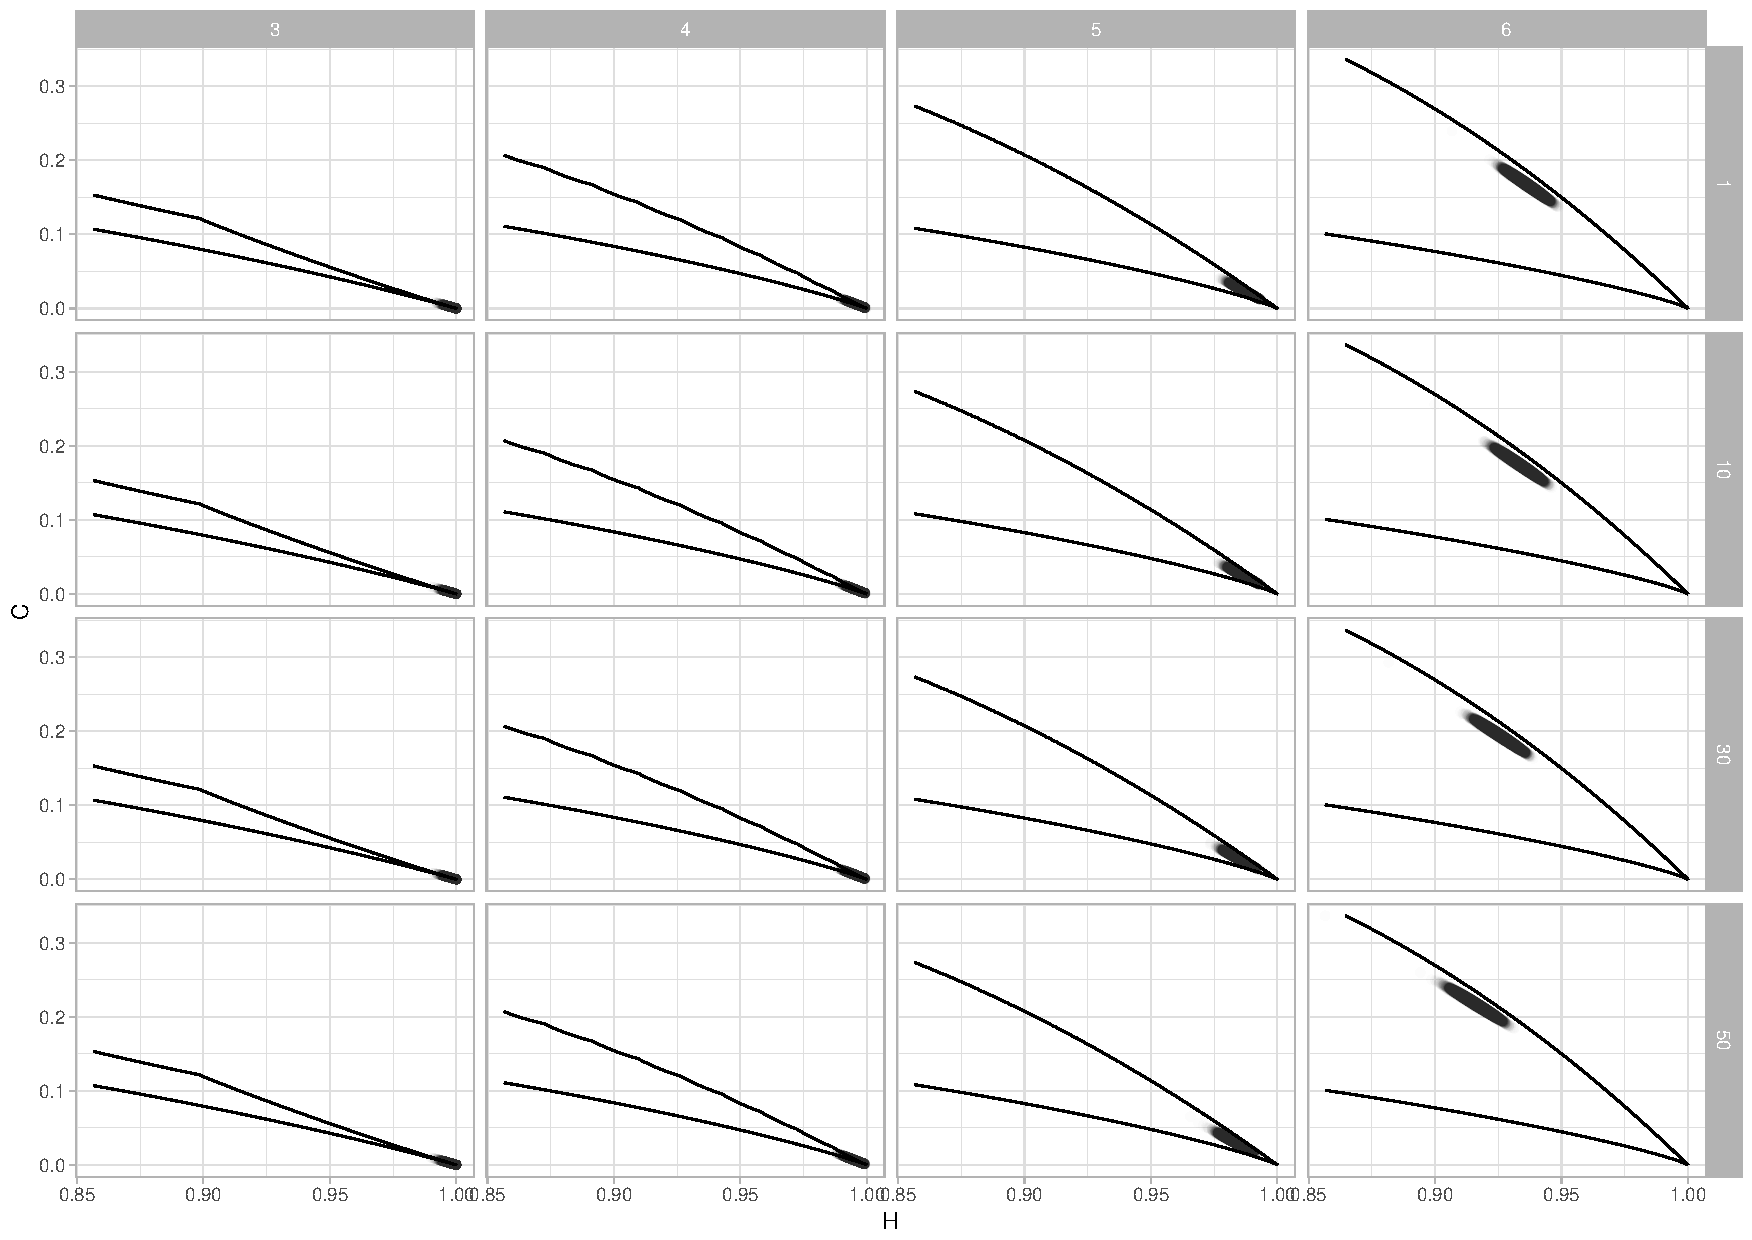
\includegraphics[width=\linewidth]{ScatterAllRandom}
%	\caption{Diagramas de dispersão das sequências de rádio para $D\in\{3,4,5,6\}$ (colunas) e $\tau\in\{1,10,30,50\}$ (linhas), com curvas de complexidade mínima e máxima no plano Entropia-Complexidade.}\label{Fig:ScatterAllRandom}
%\end{figure}
%
%A figura~\ref{Fig:ScatterAllMT} mostra os planos Entropia-Complexidade com as respectivas curvas de complexidade mínima e máxima para cada par $D\in\{3,4,5,6\}$ (colunas) e $\tau\in\{1,10,30,50\}$ (linhas), com os \num{52429} pontos observados a partir das sequências obtidas pelo gerador de Mersenne-Twister.
%Os pontos foram desenhados com \SI{1}{\percent} de transparência, para evidenciar as regiões mais e menos densas.
%
%\begin{figure}[hbt]
%	\centering
%	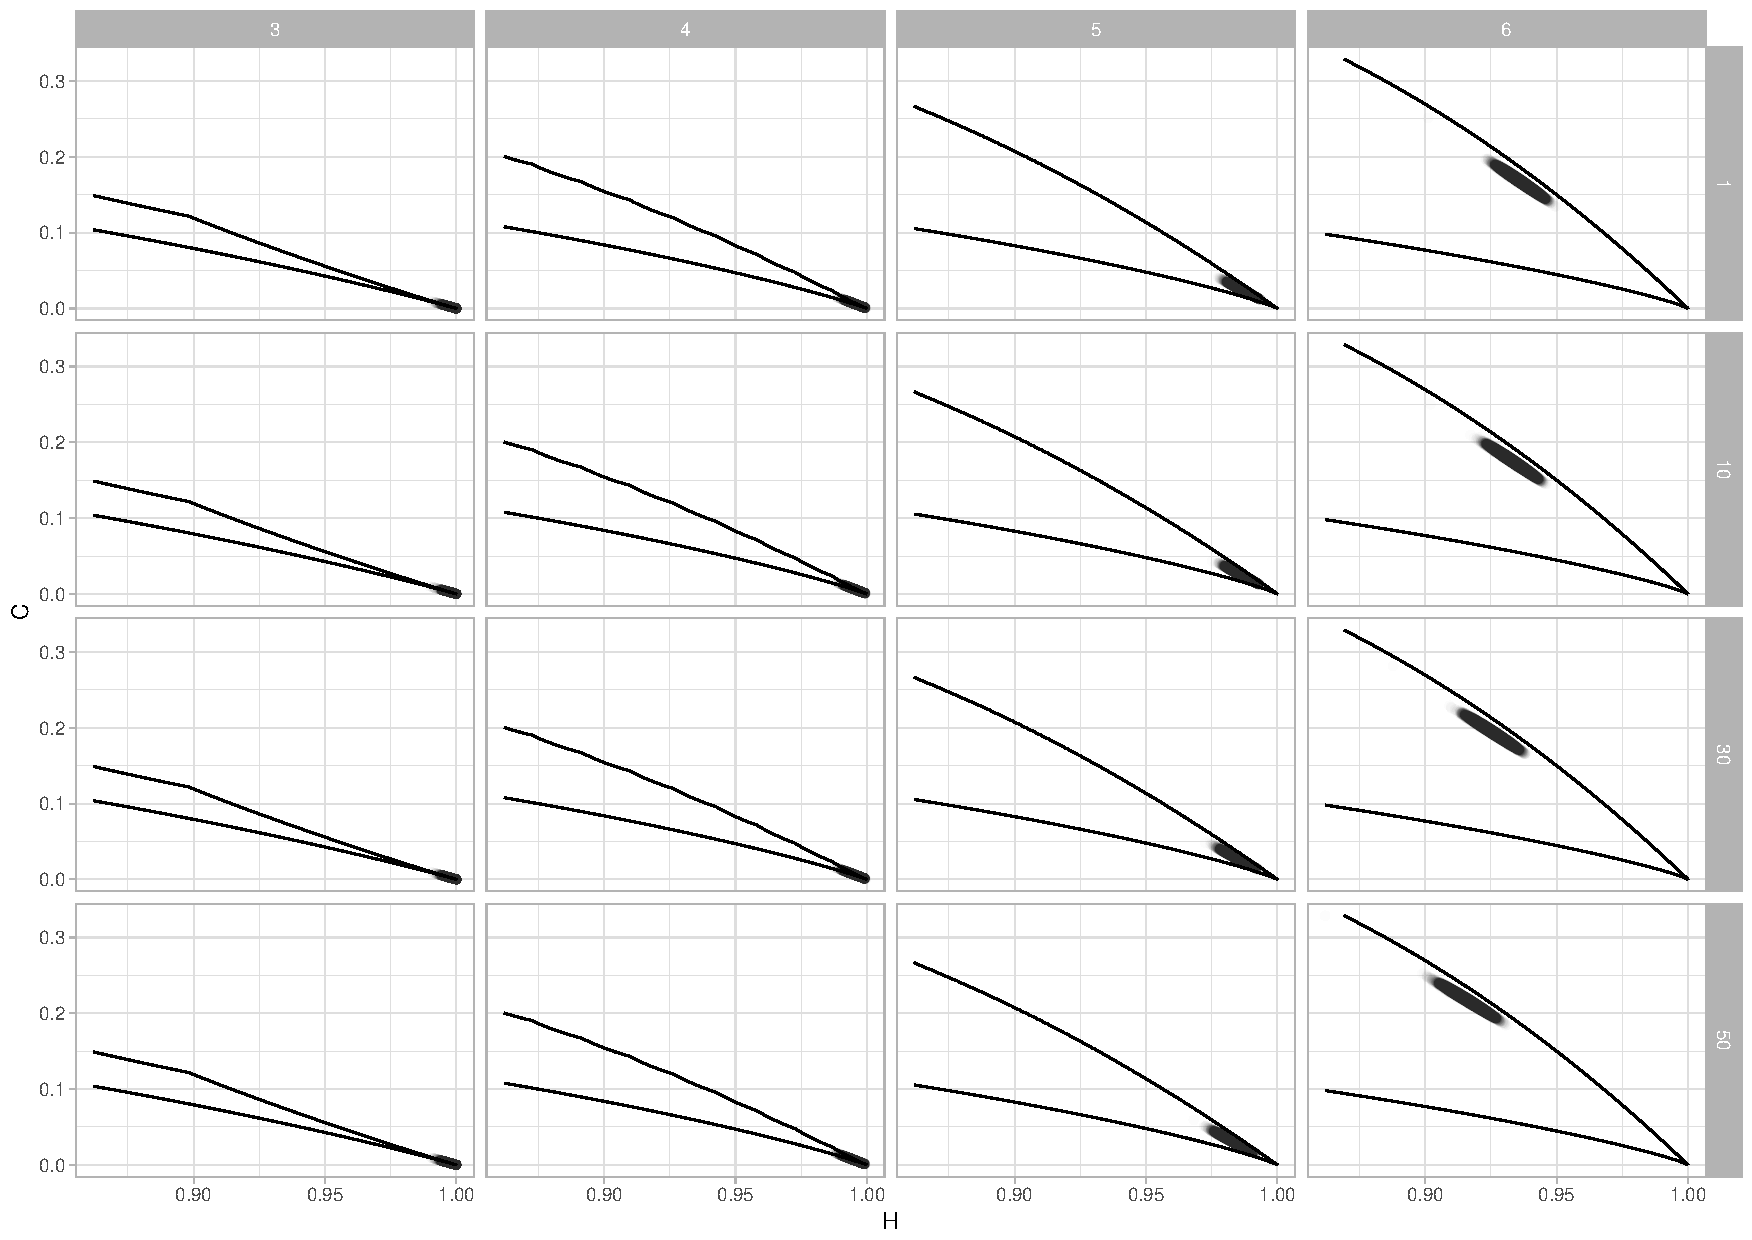
\includegraphics[width=\linewidth]{ScatterAllMT}
%	\caption{Diagramas de dispersão das sequências de Mersenne-Twister para $D\in\{3,4,5,6\}$ (colunas) e $\tau\in\{1,10,30,50\}$ (linhas), com curvas de complexidade mínima e máxima no plano Entropia-Complexidade.}\label{Fig:ScatterAllMT}
%\end{figure}

\begin{figure}[hbt]
\centering
\includegraphics[width=\linewidth]{HistoDistanciasQuantTodas}
\caption{Histogramas suavizados das distâncias euclidianas dos padrões ao ponto de referência, para $D\in\{3,4,5,6\}$ (colunas) e $\tau\in\{1,10,30,50\}$ (linhas).}\label{Fig:HistoDistanciasQuantTodas}
\end{figure}

A figura~\ref{Fig:HistoDistanciasQuantTodas} sugere que o comportamento das distâncias euclidianas ao ponto de referência muda conforme o tamanho do padrão $D$ varia.
Além disso, também são perceptíveis mudanças de comportamento em função do \textit{lag} $\tau$ quando $D=5,6$.

%A figura~\ref{Fig:HistoDistanciasRandTodas} sugere que o comportamento das distâncias euclidianas ao ponto de referência muda conforme o tamanho do padrão $D$ varia.
%Além disso, também são perceptíveis mudanças de comportamento em funçao do \textit{lag} $\tau$ quando $D=5,6$.


%\begin{figure}[hbt]
%	\centering
%	\includegraphics[width=\linewidth]{HistoDistanciasRandTodas}
%	\caption{Histogramas suavizados das distâncias euclidianas dos padrões ao ponto de referência, para $D\in\{3,4,5,6\}$ (colunas) e $\tau\in\{1,10,30,50\}$ (linhas).}\label{Fig:HistoDistanciasRandTodas}
%\end{figure}

Da análise aqui apresentada concluímos que, à luz da distância do ponto característico de uma sequência ao ponto de referência, os dois geradores físicos produzem sequências indistinguíveis.
Diante disso, nos cálculos subsequentes faremos a junção desses conjuntos de dados, que denominaremos simplesmente ``aleatórios'' no que segue.

Já o gerador de Mersenne-Twister apresenta diferenças em relação aos geradores de origem física.
Por se tratar de um gerador algorítmico e, portanto, pseudoaleatório, ele será tratado como objeto de análise e não como padrão para estabelecer critérios de qualidade.

No que segue analisaremos o comportamento dessas distâncias em detalhes.

\section{Análise das regiões de confiança}

Feita a junção das distâncias dos pontos característicos ao ponto de referência das sequências produzidas pelos geradores quântico e de rádio (sequências aleatórias), 
para cada situação de $N=1.000, 50.000$, $D=3, 4, 5, 6$ e $\tau=1, 10, 30, 50$, o próximo passo consiste em calcular os quantis relevantes.

Inicialmente ilustraremos apenas duas situações.
A figura~\ref{Fig:AleattD3tau1} mostra os padrões das sequências aleatórias para o caso $N=1.000$, $D=3$ e $\tau=1$ no plano Entropia-Complexidade, junto com os quantis de \SI{90}{\percent}, \SI{95}{\percent}, \SI{99}{\percent} e \SI{99,9}{\percent} em escala linear (figura~\ref{Fig:scatter1000D3t1}) e em escala logarítmica (figura~\ref{Fig:scatter1000D3t1_log}).

\begin{figure}
\centering
\subfigure[Escala linear\label{Fig:scatter1000D3t1}]{\includegraphics[width=.48\linewidth]{scatter1000D3t1}}
\subfigure[Escala logarítmica\label{Fig:scatter1000D3t1_log}]{\includegraphics[width=.48\linewidth]{scatter1000D3t1_log}}
\caption{Diagramas de dispersão das sequências aleatórias para o caso $N=1.000$, $D=3$ e $\tau=1$.}\label{Fig:AleattD3tau1}
\end{figure}

A figura~\ref{Fig:QuantD3tau10log} mostra os padrões das sequências aleatórias para o caso $N=50.000$, $D=6$ e $\tau=50$ no plano Entropia-Complexidade, junto com os quantis de \SI{90}{\percent}, \SI{95}{\percent}, \SI{99}{\percent} e \SI{99,9}{\percent} em escala linear (figura~\ref{Fig:scatter50kD6t50}) e em escala logarítmica (figura~\ref{Fig:scatter50kD6t50_log}).

\begin{figure}
\centering
\subfigure[Escala linear\label{Fig:scatter50kD6t50}]{\includegraphics[width=.48\linewidth]{scatter50kD6t50}}
\subfigure[Escala logarítmica\label{Fig:scatter50kD6t50_log}]{\includegraphics[width=.48\linewidth]{scatter50kD6t50_log}}
\caption{Diagramas de dispersão das sequências aleatórias para o caso $N=50.000$, $D=6$ e $\tau=50$.}\label{Fig:QuantD3tau10log}
\end{figure}

Nestas duas figuras, os pontos característicos foram desenhados com um gradiente de cores que vai do amarelo ao preto em função da distância ao ponto de referência.
Identificamos também os valores de Entropia e de Complexidade Estatística correspondentes a cada quantil de interesse.

Os resultados centrais dessa dissertação são exibidos nas figuras~\ref{Fig:Conf_Int_1k_T1}, \ref{Fig:Conf_Int_1k_T10}, 
\ref{Fig:Conf_Int_1k_30} e~\ref{Fig:Conf_Int_1k_T50} (os quantis de interesse para amostras de tamanho $1.000$ e $\tau=1, 10, 30, 50$), e nas figuras~\ref{Fig:Conf_Int_50k_T1}, \ref{Fig:Conf_Int_50k_T10},
\ref{Fig:Conf_Int_50k_30} e~\ref{Fig:Conf_Int_50k_T50} (os quantis de interesse para amostras de tamanho $50.000$ e $\tau=1, 10, 30, 50$).
Cada uma destas figuras inclui as quatro situações de $D=3, 4, 5, 6$.

%% N=1.000
\begin{figure}
	\centering
	\includegraphics[width=1\linewidth]{Conf_Int_1k_T1_noMT}
	\caption{Intervalos de confiança para o caso $N=1.000$ e $\tau=1$.}\label{Fig:Conf_Int_1k_T1}
\end{figure}

\begin{figure}
	\centering
	\includegraphics[width=1\linewidth]{Conf_Int_1k_T10_noMT}
	\caption{Intervalos de confiança para o caso $N=1.000$ e $\tau=10$.}\label{Fig:Conf_Int_1k_T10}
\end{figure}

\begin{figure}
	\centering
	\includegraphics[width=1\linewidth]{Conf_Int_1k_T30_noMT}
	\caption{Intervalos de confiança para o caso $N=1.000$ e $\tau=30$.}\label{Fig:Conf_Int_1k_30}
\end{figure}

\begin{figure}
	\centering
	\includegraphics[width=1\linewidth]{Conf_Int_1k_T50_noMT}
	\caption{Intervalos de confiança para o caso $N=1.000$ e $\tau=50$.}\label{Fig:Conf_Int_1k_T50}
\end{figure}
%%

%% N=50.000
\begin{figure}
	\centering
	\includegraphics[width=1\linewidth]{Conf_Int_50k_T1_noMT}
	\caption{Intervalos de confiança para o caso $N=50.000$ e $\tau=1$.}\label{Fig:Conf_Int_50k_T1}
\end{figure}

\begin{figure}
	\centering
	\includegraphics[width=1\linewidth]{Conf_Int_50k_T10_noMT}
	\caption{Intervalos de confiança para o caso $N=50.000$ e $\tau=10$.}\label{Fig:Conf_Int_50k_T10}
\end{figure}

\begin{figure}
	\centering
	\includegraphics[width=1\linewidth]{Conf_Int_50k_T30_noMT}
	\caption{Intervalos de confiança para o caso $N=50.000$ e $\tau=30$.}\label{Fig:Conf_Int_50k_30}
\end{figure}

\begin{figure}
	\centering
	\includegraphics[width=1\linewidth]{Conf_Int_50k_T50_noMT}
	\caption{Intervalos de confiança para o caso $N=50.000$ e $\tau=50$.}\label{Fig:Conf_Int_50k_T50}
\end{figure}
%%

Adicionalmente, aos gráficos apresentados, as tabelas \ref{tab:dEuclid_1000} e \ref{tab:dEuclid_50k} mostram os valores da distância euclidiana dos pontos de interesse dos quantis ao ponto de referência.

\begin{table}[hbt]
	\centering
	\caption{Valores das distâncias euclidianas para os valores de $D= 3, 4, 5, 6$ e $\tau=1, 10, 30, 50$ para sequências de $1.000$ observações.}\label{tab:dEuclid_1000}
	\begin{tabular}{ccccccc}
	\toprule
$N=1.000$	&  $D$  &$\tau$  &\SI{90}{\percent}&\SI{95}{\percent}&\SI{99}{\percent}&\SI{99.9}{\percent}\\
\midrule
			&  $3$ &  $ 1$ & 2.728065e-03  &  3.478919e-03  &  0.0053313857  &  0.0081048900 \\ 
			&  $3$ &  $10$ & 2.802528e-03  &  3.577539e-03  &  0.0054960059  &  0.0083091257 \\
			&  $3$ &  $30$ & 2.961344e-03  &  3.749702e-03  &  0.0056871429  &  0.0087472165 \\
			&  $3$ &  $50$ & 3.120298e-03  &  3.950138e-03  &  0.0059008109  &  0.0090272065 \\
\midrule
			&  $4$ &  $ 1$ & 7.964076e-03  &  9.015899e-03  &  0.0112777244  &  0.0143372255 \\ 
			&  $4$ &  $10$ & 8.199472e-03  &  9.295153e-03  &  0.0116255590  &  0.0147762539 \\
			&  $4$ &  $30$ & 8.738506e-03  &  9.883617e-03  &  0.0123589751  &  0.0156235388 \\
			&  $4$ &  $50$ & 9.368242e-03  &  1.054840e-02  &  0.0131188349  &  0.0166817556 \\
\midrule
			&  $5$ &  $ 1$ & 3.117067e-02  &  3.304803e-02  &  0.0366895915  &  0.0413215927 \\ 
			&  $5$ &  $10$ & 3.235895e-02  &  3.425898e-02  &  0.0380480169  &  0.0427998033 \\
			&  $5$ &  $30$ & 3.545788e-02  &  3.752600e-02  &  0.0417425086  &  0.0467667352 \\
			&  $5$ &  $50$ & 3.914194e-02  &  4.142425e-02  &  0.0459567507  &  0.0514563584 \\
\midrule
			&  $6$ &  $ 1$ & 1.891794e-01  &  1.923893e-01  &  0.1984529319  &  0.2050583463 \\
			&  $6$ &  $10$ & 1.975446e-01  &  2.007669e-01  &  0.2069269144  &  0.2139321164 \\
			&  $6$ &  $30$ & 2.185870e-01  &  2.218804e-01  &  0.2280312709  &  0.2345272440 \\
			&  $6$ &  $50$ & 2.431686e-01  &  2.464034e-01  &  0.2526103765  &  0.2596196960 \\
	\bottomrule
\end{tabular}
\end{table}

\begin{table}[hbt]
	\centering
	\caption{Valores das distâncias euclidianas para os valores de $D= 3, 4, 5, 6$ e $\tau=1, 10, 30, 50$ para sequências de $50.000$ observações.}\label{tab:dEuclid_50k}
	\begin{tabular}{ccccccc}
		\toprule
$N = 50.000$	&  $D$  &$\tau$  &\SI{90}{\percent}&\SI{95}{\percent}&\SI{99}{\percent}&\SI{99.9}{\percent}\\ 
\midrule
				&  $3$  &  $ 1$  &  5.407679e-05  &  7.015910e-05  &  0.0001178519  &  0.0001917689 \\ 
				&  $3$  &  $10$  &  5.636160e-05  &  7.130762e-05  &  0.0001000853  &  0.0001585019 \\
				&  $3$  &  $30$  &  5.731458e-05  &  7.245769e-05  &  0.0001101931  &  0.0001580179 \\
				&  $3$  &  $50$  &  5.951595e-05  &  7.541980e-05  &  0.0001093136  &  0.0001983728 \\ 
\midrule
				&  $4$  &  $ 1$  &  1.589081e-04  &  1.818144e-04  &  0.0002250318  &  0.0003038889 \\ 
				&  $4$  &  $10$  &  1.588585e-04  &  1.790301e-04  &  0.0002264259  &  0.0002903681 \\
				&  $4$  &  $30$  &  1.631504e-04  &  1.863802e-04  &  0.0002330694  &  0.0002893557 \\
				&  $4$  &  $50$  &  1.619028e-04  &  1.809200e-04  &  0.0002311957  &  0.0003017229 \\ 
\midrule
				&  $5$  &  $ 1$  &  6.062508e-04  &  6.389830e-04  &  0.0007179730  &  0.0008832568 \\ 
				&  $5$  &  $10$  &  5.985032e-04  &  6.289105e-04  &  0.0007041024  &  0.0007855387 \\
				&  $5$  &  $30$  &  6.040569e-04  &  6.400727e-04  &  0.0007268196  &  0.0008213228 \\
				&  $5$  &  $50$  &  6.055769e-04  &  6.381391e-04  &  0.0007134216  &  0.0008042788 \\ 
\midrule
				&  $6$  &  $ 1$  &  3.071590e-03  &  3.150152e-03  &  0.0033104814  &  0.0035923810 \\ 
				&  $6$  &  $10$  &  3.050841e-03  &  3.117779e-03  &  0.0032553996  &  0.0033734229 \\
				&  $6$  &  $30$  &  3.066360e-03  &  3.129649e-03  &  0.0032669327  &  0.0034581195 \\
				&  $6$  &  $50$  &  3.074748e-03  &  3.147889e-03  &  0.0032828968  &  0.0034178859 \\
		\bottomrule
	\end{tabular}
\end{table}
\mychapter{Conclusão}{chp:conclusao}
\lhead{CONCLUSÃO}

Neste trabalho analisamos a possibilidade de a distância euclidiana de pontos no plano $(H\times C)$ de sequências ao ponto $(1,0)$, referência teórica de ruído branco, poderem ser usadas como uma estatística de teste para a hipótese de a sequência ser ruído branco.
Verificamos que essa possibilidade existe, e que essa estatística é capaz de identificar, com limitações, o mapa logístico (que já foi usado como gerador de números pseudoaleatórios), movimento browniano e ruído com autocorrelação.
Para este último, fizemos uma análise preliminar do poder do teste em função da intensidade da correlação.

Verificamos, também, que os geradores Mersenne-Twister e Randu são considerados ruído branco, mesmo sendo eles técnicas algorítmicas de geração de observações pseudoaleatórias.

%A técnica permite discriminar observações de ruído browniano (não estacionário), do mapa logístico e, com limitações, de ruído estacionário obtido pela convolução de uma sequência de ruído branco com uma máscara.
Sendo a máscara parametrizada, fizemos uma análise preliminar do poder do teste.

Uma limitação deste trabalho é que apenas verificamos a qualidade do gerador em relação a um de estrutura ideal.
Com isso, limitamos a aplicabilidade do nosso trabalho à análise de séries que, potencialmente, são ocorrências de variáveis aleatórias independentes e identicamente distribuídas.

Há farta literatura que caracteriza diferentes tipos de estruturas como, por exemplo, processos estocásticos do tipo $f^{-k}$.
A nossa metodologia pode, em princípio, ser aplicada a quaisquer processos mas, para isso, é necessário o conhecimento da distribuição dos padrões ordinais do processo de referência.
No nosso caso, trata-se da lei uniforme sobre os padrões, que é característica de ruído branco.
Não conhecemos resultados que caracterizem de forma teórica as leis de outros processos.

Há, contudo, uma solução para esse problema: estimar a lei característica do padrão de interesse.
Isso pode ser feito através de estudos Monte Carlo, mas tal extensão foge ao objetivo deste trabalho.


\appendix

\chapter{Apêndice 1 - Agoritmos}\label{codigo}


\begin{lstlisting}[language=R, caption={Mersenne Twister}, label=code:MersenneTwister]
set.seed(1234567890, kind = "Mersenne-Twister")

MT1k <- runif(1000)
MT50k <- runif(50000)
\end{lstlisting}

\begin{lstlisting}[language=R, caption={Randu}, label={code:Randu}]
RANDU <- function() {
seed <<- ((1103515245 * seed) + 12345 ) %% (2^31)
}

Randu1k <- vector()
for(i in 1:1000) {

Randu1k[i] <- c(RANDU())
}
\end{lstlisting}


\begin{lstlisting}[language=R, caption={Não Estacionária}, label={code:NaoEstacionaria}]
NoEst1k <- diffinv(rnorm(1000))
NoEst1k <- abs(NoEst1k/max(NoEst1k))

NoEst50k <- diffinv(rnorm(50000))
NoEst50k <- abs(Randu50k/max(NoEst50k))
\end{lstlisting}


\begin{lstlisting}[language=R, caption={Estacionária}, label={code:Estacionaria}]
Est1k <- filter(rnorm(1000), filter=rep(1,3), circular=TRUE)

Est50k <- filter(rnorm(50000), filter=rep(1,3), circular=TRUE)
\end{lstlisting}


\begin{lstlisting}[language=R, caption={Mapa Logístico}, label={code:MapaLogistico}]
logisticmap <- function(N, x0) {

saida <- vector(mode="double", length=10000)
saida[1] <- x0

for(i in 2:10000)
saida[i] <- 4 * saida[i-1] * (1 - saida[i-1])

x0 <- saida[10000]
saida <- vector(mode="double", length=N)
saida[1] <- x0

for(i in 2:N)
saida[i] <- 4 * saida[i-1] * (1 - saida[i-1])

return(saida)
}

LogMap1k <- logisticmap(1000, .01)
LogMap50k <- logisticmap(50000, .01)

\end{lstlisting}


\begin{lstlisting}[language=R, caption={}, label={code:}]

\end{lstlisting}


% Apêndices e Anexos
\appendix
% % \mychapter{\textsc{Ambiente Reprodutível e Computacional}}{app:ambiente}
\chapter{\textsc{Ambiente Reprodutível e Computacional}}~\label{app:ambiente}
\lhead{\textsc{Ambiente Reprodutível e Computacional}}


\lettrine{O}{} \citet{ISI2012} 

%======================================================%
%============= REFERÊNCIAS BIBLIOGRÁFICAS =============%
%======================================================%
\begin{raggedright}
\renewcommand{\bibsection}{
\chapter*{\vspace{-3cm}\centering \Large \textsc{Referências Bibliográficas}}
\addcontentsline{toc}{chapter}{Referências Bibliográficas}
}
\lhead{\textsc{Referências Bibliográficas}}
\bibliography{references}
\newpage\lhead{\rightmark}
\end{raggedright}

%======================================================%

\chapter*{}
\vfill
\singlespacing
\thispagestyle{empty}
\begin{center}
\includegraphics[width=.3\textwidth]{./capitulos/figs/knot}

\vspace{.5cm}

Este trabalho foi redigido em {\large \LaTeX}\ utilizando uma modificação do estilo \textsf{IC-UFAL}.
As referências bibliográficas foram preparadas no \textsf{JabRef} e administradas pelo {\large\BibTeX}\ com o estilo \textsf{LaCCAN}.
O texto utiliza fonte \NomeFonte\ e os elementos matemáticos a família tipográfica \NomeFonteMat, ambas em corpo de 12 pontos.
% A numeração dos capítulos segue com a família tipográfica \NomeFonteCap.\\ 
\vspace{.5cm}
%
\includegraphics[width=.5\textwidth]{./capitulos/figs/celtic_knot_cross_stitch}
\end{center}

\end{document}
